\begin{itemize}
    \item Joins are used to combine rows from two or more tables based on a related column between them.
    \item Used to combine tables to consolidate a result.
    
    \item We want to know the names and employee id of each of the branches.
        \begin{minted}[autogobble]{sql}
            SELECT employee.emp_id, employee.first_name, branch.branch_name 
            FROM employee JOIN branch ON employee.emp_id = branch.mgr_id;
        \end{minted}
        \begin{figure}[H]
            \centering
            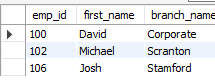
\includegraphics[width=0.4\textwidth]{./figs/JOINS.png}
        % 	\caption{\href{}{source}}
        \end{figure}
    
    \item Left joins:
        \begin{itemize}
            \item On a left join all of the table is included but only the one that matches.
        \end{itemize}
        \begin{minted}[autogobble]{sql}
            SELECT employee.emp_id, employee.first_name, branch.branch_name 
            FROM employee LEFT JOIN branch ON employee.emp_id = branch.mgr_id;
        \end{minted}
        \begin{figure}[H]
            \centering
            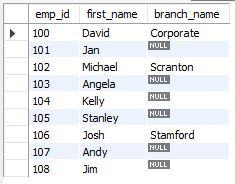
\includegraphics[width=0.4\textwidth]{./Figs/2020-12-24-21-05-22.png}
        % 	\caption{}
        \end{figure}
    
    \item Right join:
        \begin{minted}[autogobble]{sql}
            SELECT employee.emp_id, employee.first_name, branch.branch_name 
            FROM employee RIGHT JOIN branch ON employee.emp_id = branch.mgr_id;
        \end{minted}
        \begin{figure}[H]
            \centering
            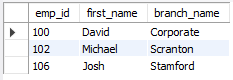
\includegraphics[width=0.4\textwidth]{./Figs/2020-12-24-21-05-51.png}
        % 	\caption{}
        \end{figure}
    
    \item There is an outer join but this is not available in mysql.
\end{itemize}

